% !TEX program = xelatex
\documentclass[12pt]{article}
\usepackage[margin=1in]{geometry}
\usepackage{nopageno} % no page numbers
\usepackage{setspace} \doublespacing

\usepackage{graphicx}
\graphicspath{ {./graphics/} }
\usepackage[dvipsnames]{xcolor}
\definecolor{CrispBlue}{HTML}{0176AE}

\usepackage{fontspec}
\usepackage{tcolorbox}
\usepackage{etoolbox}
\BeforeBeginEnvironment{verbatim*}{\begin{tcolorbox}[colback=CrispBlue!5!white,colframe=CrispBlue!75!black]}%
\AfterEndEnvironment{verbatim*}{\end{tcolorbox}}%

\usepackage{hyperref}
\hypersetup{
    colorlinks,
    citecolor=black,
    filecolor=black,
    linkcolor=black,
    urlcolor=black
}

\renewcommand{\footnotesize}{\fontsize{8pt}{10pt}\selectfont}


\usepackage[labelfont={small,sc,bf},textfont={small,sc,bf}]{caption}
\setlength{\parindent}{24pt}
% \setlength{\parskip}{1em}

\usepackage{tocloft}
\renewcommand{\cftpartleader}{\cftdotfill{\cftdotsep}}
\renewcommand{\cftsecleader}{\cftdotfill{\cftdotsep}}

\usepackage[shortlabels]{enumitem}

\usepackage{lastpage}
\usepackage{fancyhdr}
\pagestyle{fancy}
\fancyhf{}
\renewcommand{\headrulewidth}{0pt}
\rfoot{Page \thepage\ of \pageref*{LastPage}}

\usepackage{amsmath,amsfonts,amssymb}
\usepackage{bm}
\usepackage{mathtools}

\renewcommand{\listfigurename}{List of Figures}

\begin{document}
\setmainfont{SF Pro Text}
\setsansfont{SF Pro Text}
\setmonofont{SF Mono}
\renewcommand{\familydefault}{\sfdefault}

\hypersetup{
    linkcolor=CrispBlue,
    urlcolor=CrispBlue,
    breaklinks=true
}

\noindent David Kirby\\
ECE 595: Advanced Technical Cybersecurity\\
Spring, 2022
\begin{center}
    \large\bfseries Comparing Ciphers
\end{center}

This paper compares the ciphers we have discussed in class (i.e., the Caesar cipher, the Vigen\`ere cipher, and the bifid cipher). We compare the resulting ciphertexts and plaintexts based on a variety of inputs and outputs, focusing on varying input string lengths and types. We discuss the strengths and weaknesses of each cipher and their complexities to implement.

We begin our discussion of the Vigen\`ere cipher by first detailing columnar transpositions. Columnar transposition ciphers use a keyword that is going to be selected prior to the enciphering or deciphering step, and we are going to need to have the same keyword to encipher and decipher. We can also use a pad of keywords, whereby we use a keyword to encipher a message, use that same keyword to decipher the message, and then never use that keyword again. This method was used extensively during World War II\footnote{\href{https://learning.oreilly.com/library/view/real-world-python/9781098125721/xhtml/ch04.xhtml}{https://learning.oreilly.com/library/view/real-world-python/9781098125721/xhtml/ch04.xhtml}}; for example, the Germans used the novel \textit{Rebecca} as a code book where the sender and receiver have a copy of the book, then, after one use, the top sheet is torn off and discarded. These so-called one-time pads provided nearly unbreakable encryption for many years, but they require a key that is at least the same length as the message being enciphered (see the running key example in Figure~\ref{fig:error}). Also paramount is the need to secure the one-time pads. In order to use columnar ciphers, as the name suggests, we are going to create a columnar structure with the keyword on top and we are going to put the message along the bottom and alphabetize the keyword. When we alphabetize the keyword, we transpose all of the columns accordingly with the key.

\begin{figure}[!ht]
    \centering
    \includegraphics[width=0.5\textwidth]{512px-Vigenère_square_shading.png}
    \caption{Tabula recta.}
    \label{fig:tabula}
\end{figure}

These columnar ciphers lead us next to discuss Vigen\`ere ciphers, a polyalphabetic substitution cipher that uses a very large lookup table called a tableau or tabula recta. This tabula recta (see Figure~\ref{fig:tabula}) contains essentially the alphabet shifted by one letter in each column, so the first column is \(A\), \(B\), \(C\) through \(Z\) the next column is \(B\), \(C\), \(D\) \ldots\ with \(A\) at the end column. We index into this to be able to come up with our ciphertext as well as index into this to decipher. The crucial part is, we repeat the keyword along the top as many times as we have letters from the message (sans spaces). Doing this we create a pair, for example we have \(K, T\), which indexes to \(D\). We repeat this step for every letter-pair, reversing the process to decipher. The running key cipher is very similar to the Vigen\`ere cipher in that it uses the tabula recta, but with the difference being that the key is much longer. Vigen\`ere repeats a single keyword as many times as it takes, running key uses a phrase, but this phrase must be at least as long as the message. As shown in Figure~\ref{fig:error}, our submitted plaintext is longer than our key, and therefore causes an error. By comparison, we see in Figure~\ref{fig:vignere} that the Vigen\`ere cipher handled the longer message string just fine. Even though the running key cipher is limited in this way, one benefit is if you never repeat the key and the key doesn't repeat inside of the ciphertext it's very difficult to decrypt.

\begin{figure}[!ht]
    \centering
    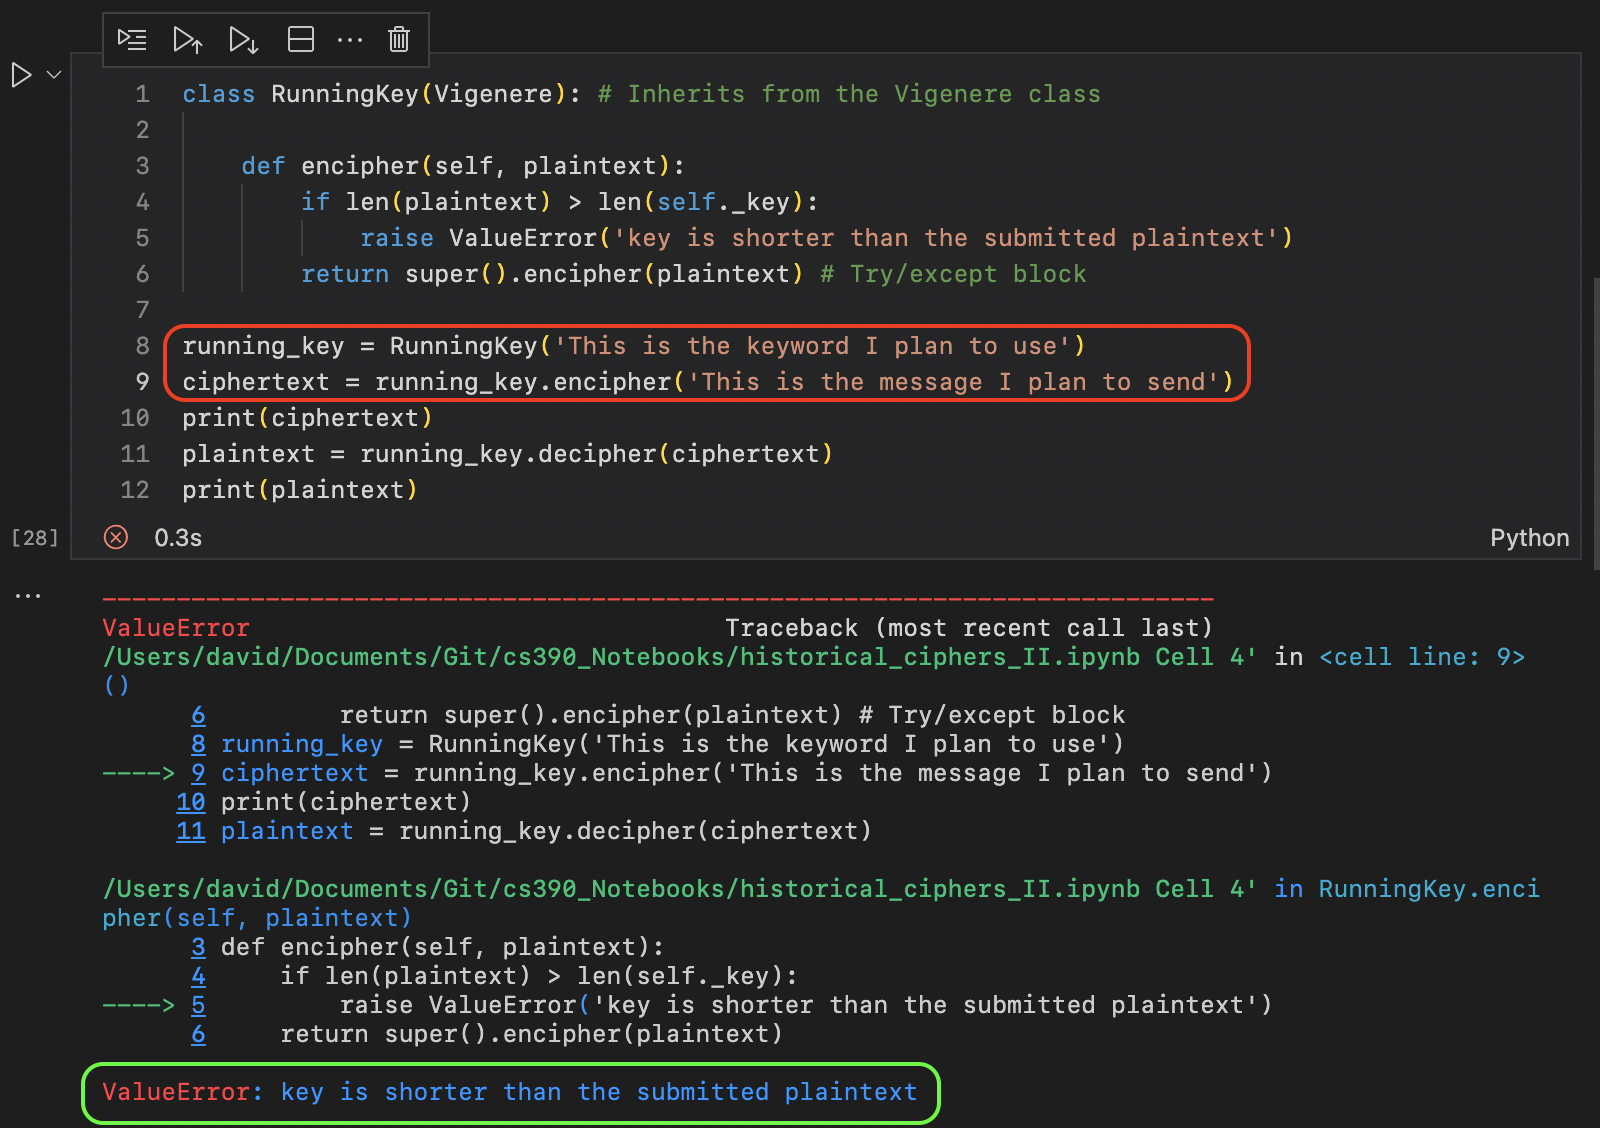
\includegraphics[width=0.8\textwidth]{figure01.png}
    \caption{Running key length error.}
    \label{fig:error}
\end{figure}

\begin{figure}[!ht]
    \centering
    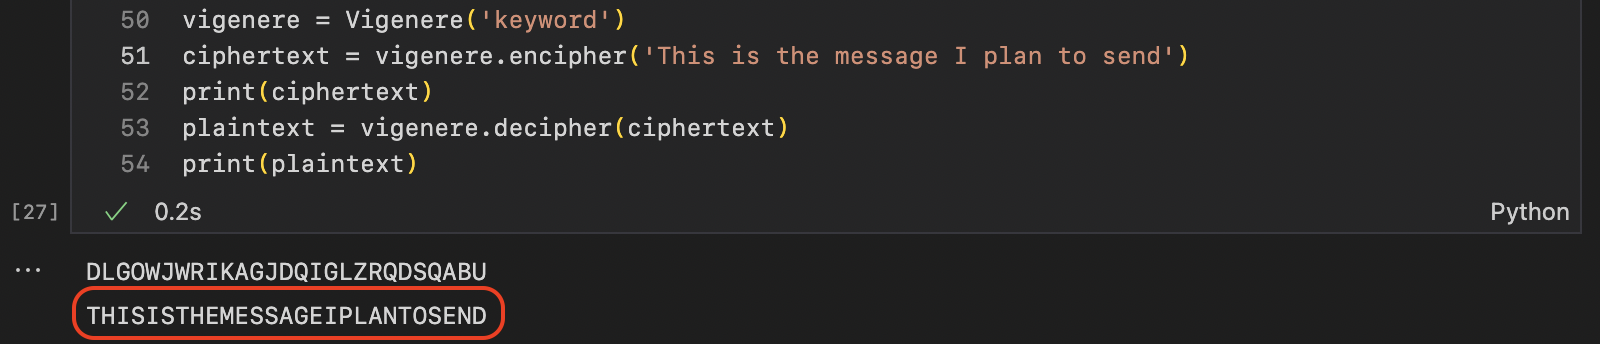
\includegraphics[width=0.8\textwidth]{figure02.png}
    \caption{Vigen\`ere running same message length.}
    \label{fig:vignere}
\end{figure}

The bifid cipher uses a key square, and inside of this key square we find numbers associated with a letter. They generally merge \(I\) with \(J\) in the square so we have a five by five square. We place coordinates vertically, transpose horizontally, and then read the coordinates horizontally to transform into letters. The coordinates of the letter in the key square are arranged vertically, the row is on top, the column is on the bottom, then we group this in groups of five called periods. One of the key characteristics of the bifid cipher is that changing the plaintext can change multiple characters of the ciphertext -- an example of diffusion. Figures~\ref{fig:bifid} and~\ref*{fig:vignere2} show a comparison of bifid cipher and the Vigen\`ere cipher, repsectively. We can see that if we pass the plaintext string \texttt{AAAAAAA} to our implementation of the Vigen\`ere cipher, we can actually retrieve the keyword used to encipher the text.

\begin{figure}[!ht]
    \centering
    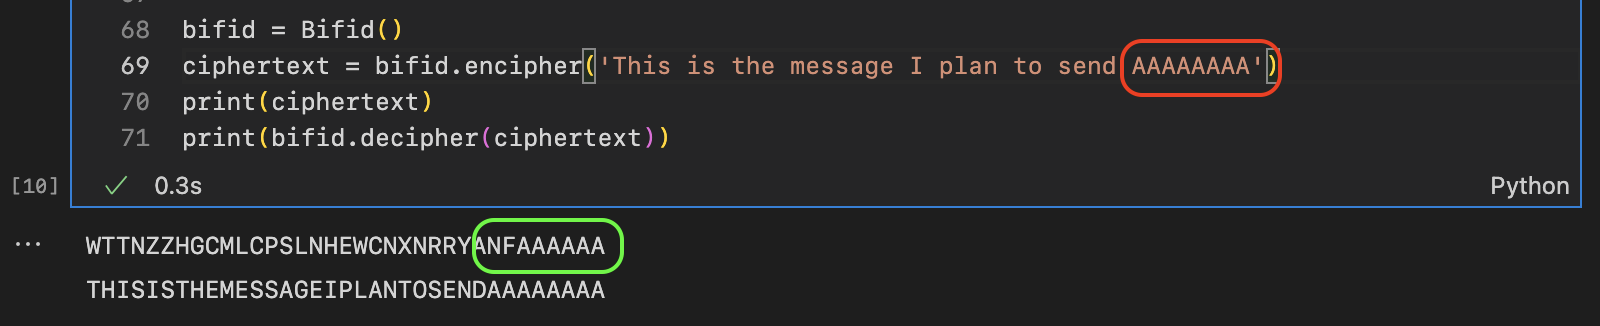
\includegraphics[width=0.90\textwidth]{figure03.png}
    \caption{Results of enciphering AAAAAAA using bifid.}
    \label{fig:bifid}
\end{figure}

\begin{figure}[!ht]
    \centering
    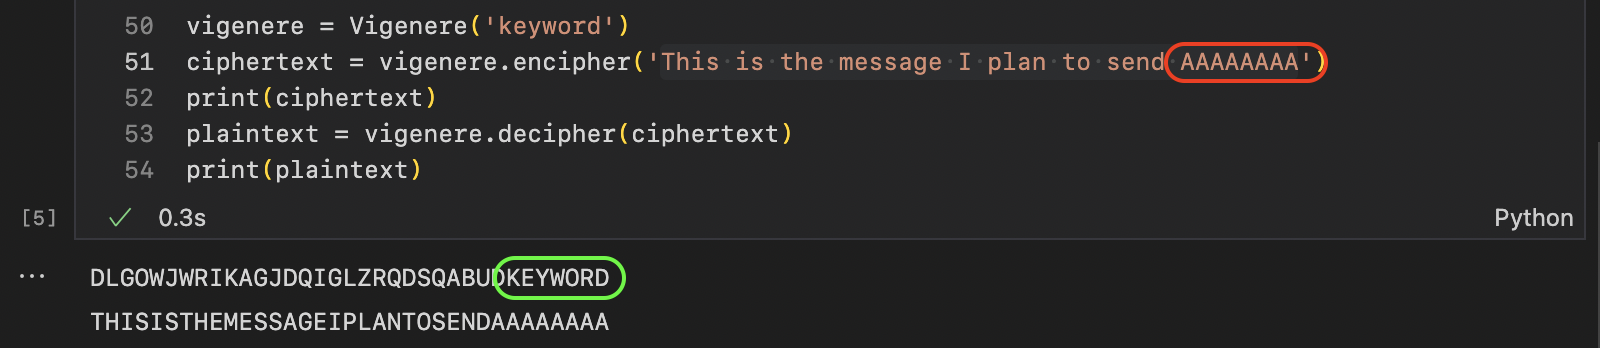
\includegraphics[width=0.9\textwidth]{figure04.png}
    \caption{Results of enciphering AAAAAAA using Vigen\`ere.}
    \label{fig:vignere2}
\end{figure}

\end{document}